\section{Ejercicio 1: Crear relaciones - Tarea 1: Relaciones automáticas} 



\begin{enumerate}[1.]
	\item  Ingresar a Power BI Desktop. En la Ventana de Power BI Desktop, click en Obtener Datos (Get Data). En el cuadro de dialogo Obtener Datos (Get Data), asegurarse que Excel esta seleccionado y hacer click en Conectar (Connect).
	En el cuadro de dialogo Abrir (Open), buscar el archivo Adventure Works Sales Data.xlsx, y luego hacer
click en Abrir (Open).	 En el cuadro de dialogo Explorador (Navigator), seleccionar las hojas DimCurrency, DimCustomer,
DimDate, DimProduct, DimPromotion, DimSalesTerritory, y FactInternetSales.
	
	

	\begin{center}
	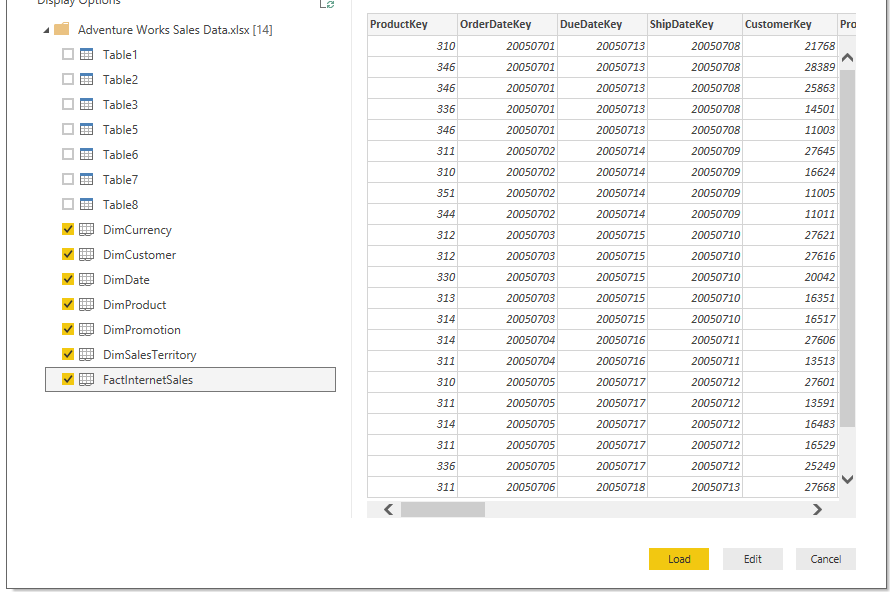
\includegraphics[width=11cm]{./Imagenes/11} 
	\end{center}


	\item   En el panel de vistas a mano derecho, hacer click en Relaciones (Relationships).
 En el menú principal, hacer click en Administrar relaciones (Manage Relationships).

	\begin{center}
	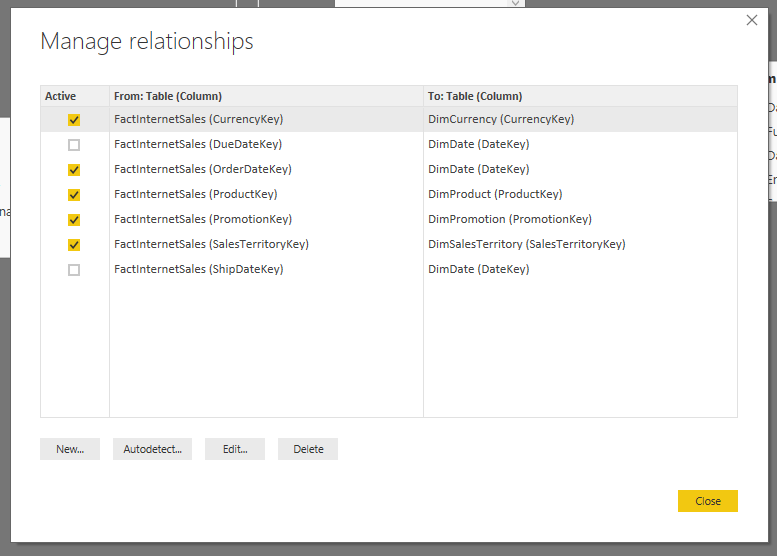
\includegraphics[width=11cm]{./Imagenes/12} 
	\end{center}



\item En el menú principal, hacer click en Administrar relaciones (Manage Relationships). En el cuadro de Administrar relaciones (Manage Relationships), hacer click en Nueva (New). En la lista de tablas superior, hacer click en FactInternetSales. Luego hacer click en la columna CustomerKey en la vista de datos previa. En la lista de tablas superior, hacer click en DimCustomer, y hacer click CustomerKey en la vista de datos previa. En la lista de Cardinalidad (Cardinality), hacer click en Muchos a Uno (Many to One (*:1)), y luego hacer click en Aceptar (OK).
	\begin{center}
	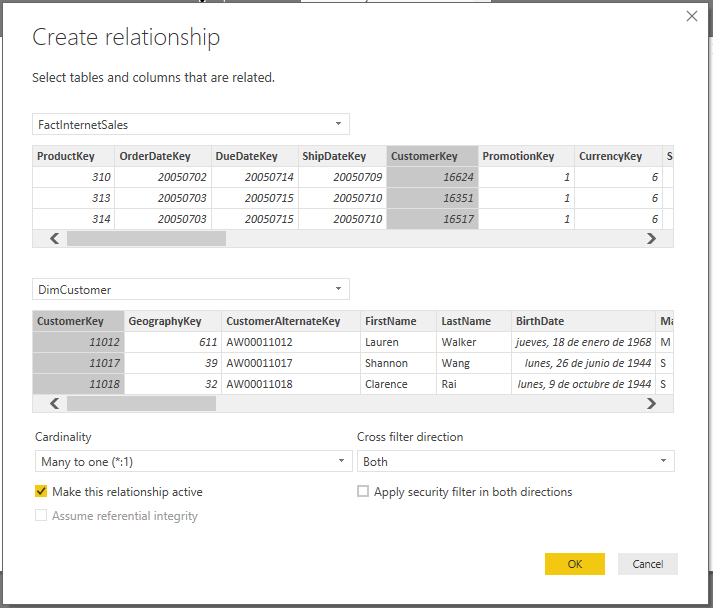
\includegraphics[width=12cm]{./Imagenes/13} 
	\end{center}

\item Cargar el archive como Ventas Adventure Works.pbix.
	\begin{center}
	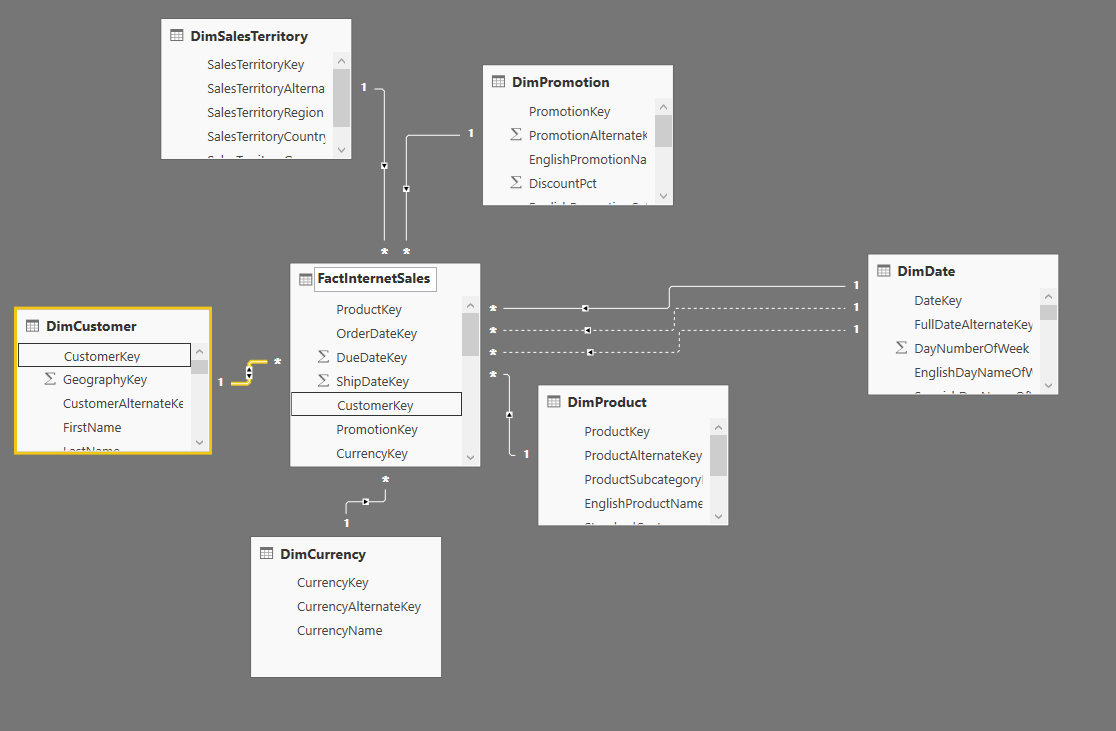
\includegraphics[width=12cm]{./Imagenes/14} 
	\end{center}

\end{enumerate}




